% visualisierung.tex
Wird der \texttt{visualize} Parameter bei der Ausführung einer R-Paket Funktion auf \texttt{TRUE} gesetzt, wird ein \texttt{RMarkdown}-Skript ausgeführt. Dieses generiert eine  Präsentation vom \LaTeX -Dokumenttyp Beamer mit Informationen und Visualisierungen zur ausgeführten Funktion.
\\
Die erzeugten Präsentationen liegen innerhalb des Programmverzeichnisses von R im Installationsordner des Pakets. Dort gibt es den \emph{pdf} Order in dem sich die Dokumente befinden. Möchte man die Dokumente vom RStudio aus öffnen, anstatt die Dokumente in der Verzeichnisstruktur suchen zu müssen, kann die \texttt{ConvOpenPDF}-Funktion (siehe Kapitel~\ref{kapitel:interface_ConvOpenPDF}) verwendet werden. Möchte man die Dokumente zu einem späteren Zeitpunkt erneut einsehen wird empfohlen eine Kopie der Datei abzuspeichern, da bei einer erneuten Ausführung der gleichen Funktion inklusive Visualisierung das zuvor erzeugte Dokument im \emph{pdf} Ordner überschrieben wird. Die vom \texttt{RMarkdown}-Skript erzeugten \LaTeX -Dateien aus denen die Beamer Präsentationen generiert werden liegen ebenfalls im selben Verzeichnis.
\\
Bei den folgenden Beispielen der Visualisierungen wurde stets punktiert, da ohne Punktierung die Informationen in den Präsentationen dazu fehlen und somit auch nicht erläutert werden können.
\\
\\
Der weitere Kapitelinhalt setzt sich folgendermaßen zusammen: [TODO]
\section{Kodierung}
\label{kapitel:visualisierung_kodierung}
% allg. Informationen
\begin{figure}[t]
	\centering
	\begin{subfigure}{0.48\textwidth}
		\centering
		\fbox{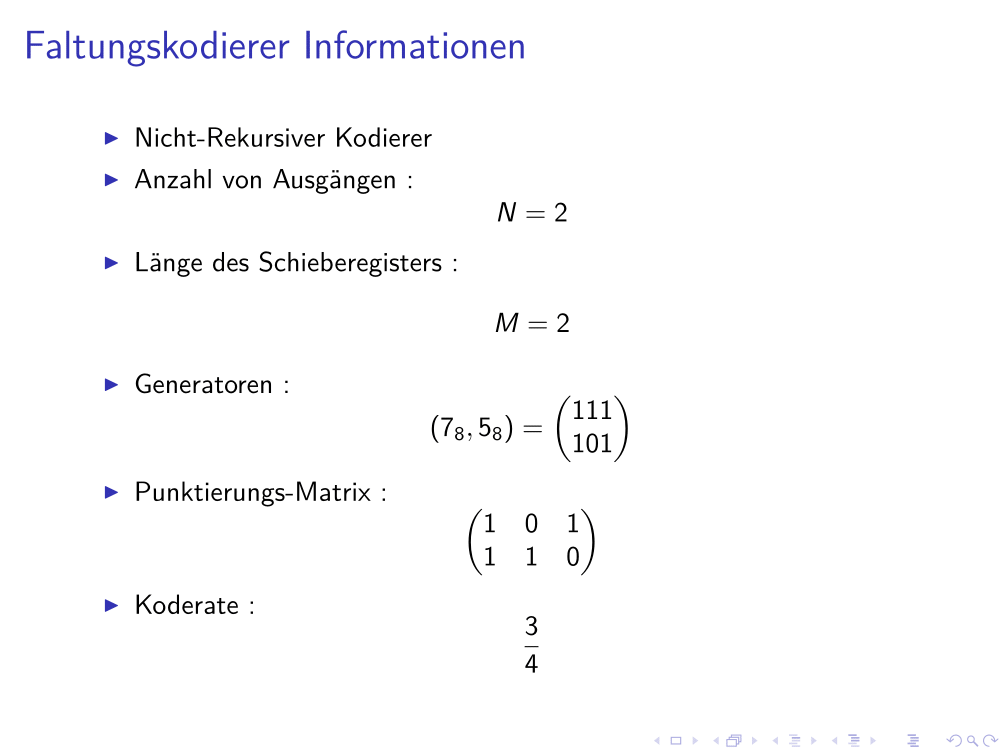
\includegraphics[width=0.99\textwidth]{abbildungen/folie_kodierung_info}}
		\caption{Folie mit Kodierer-Kennwerten}
		\label{abb:folie_kodierer_kennwerte}
	\end{subfigure}
	\quad % spacing between subfigures
	\begin{subfigure}{0.48\textwidth}
		\centering
		\fbox{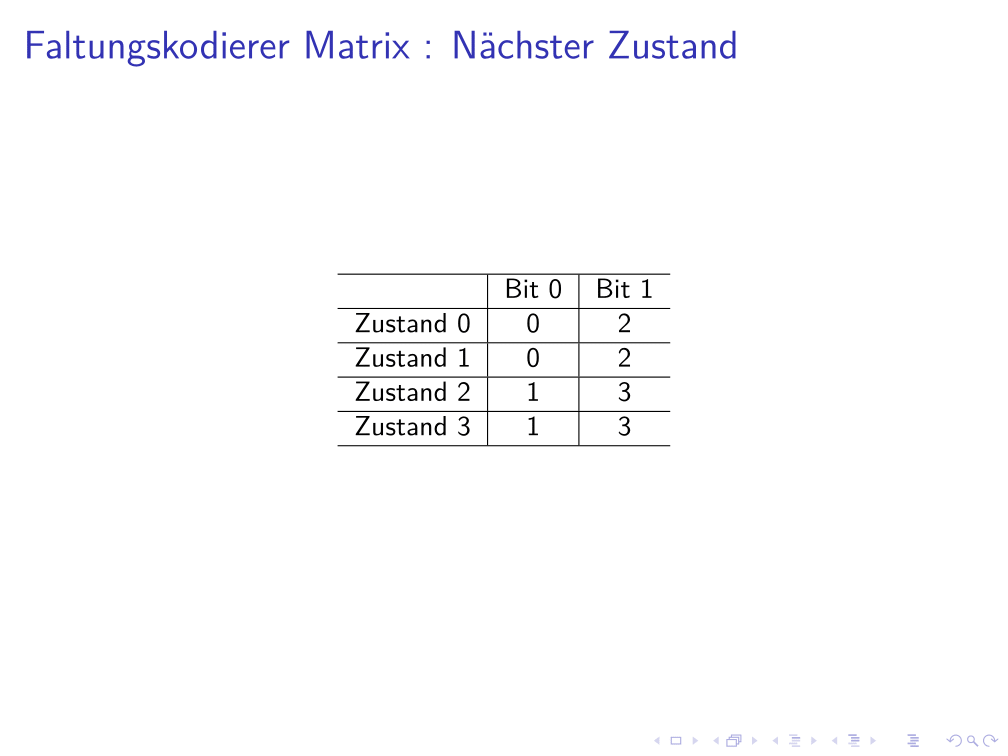
\includegraphics[width=0.99\textwidth]{abbildungen/folie_kodierung_matrix_zustand}}
		\caption{Folie mit Zustandsübergangsmatrix}
		\label{abb:folie_zustandsübergangsmatrix}
	\end{subfigure}
	\caption{Folien mit allgemeinen Informationen zum Faltungskodierer}
	\label{abb:folie_allg_info_kodierer}
\end{figure}
Bei der Kodierung befinden sich auf den ersten Folien allgemeine Informationen zum verwendeten Faltungskodierer. Abbildung~\ref{abb:folie_kodierer_kennwerte} zeigt die Folie mit den Kennwerten des Faltungskodierers: Anzahl an Ausgänge $N$, Länge des Schieberegisters $M$, Generatorpolynome, Punktierungsmatrix und Koderate. Auf den nächsten beiden Folien werden die Zustandsübergangsmatrix und die Ausgabematrix abgebildet. In Abbildung~\ref{abb:folie_zustandsübergangsmatrix} ist die Folie der Zustandsübergangsmatrix zu sehen. Analog dazu wird die Ausgabematrix auf der nächsten Folie veranschaulicht. Diese wird aus Platzgründen hier nicht abgebildet.
\\
\\
% Kodierung
\begin{figure}[t]
	\centering
	\begin{subfigure}{0.48\textwidth}
		\centering
		\fbox{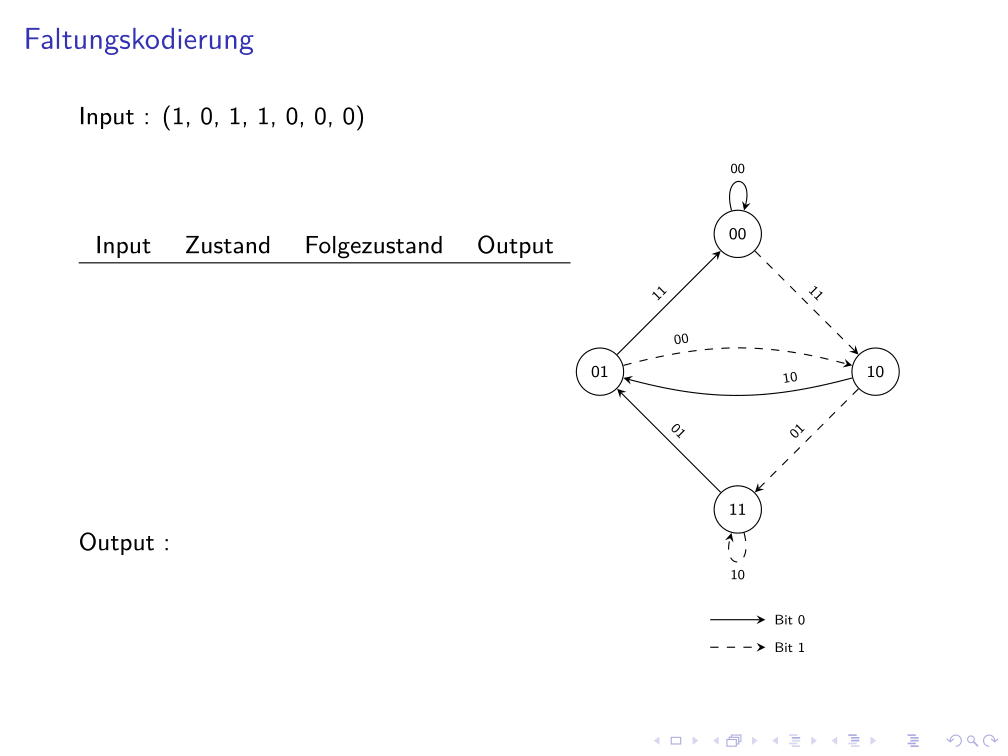
\includegraphics[width=0.99\textwidth]{abbildungen/folie_kodierung_1}}
		\caption{}
		\label{abb:folie_kodierung_1}
	\end{subfigure}
	\quad % spacing between subfigures
	\begin{subfigure}{0.48\textwidth}
		\centering
		\fbox{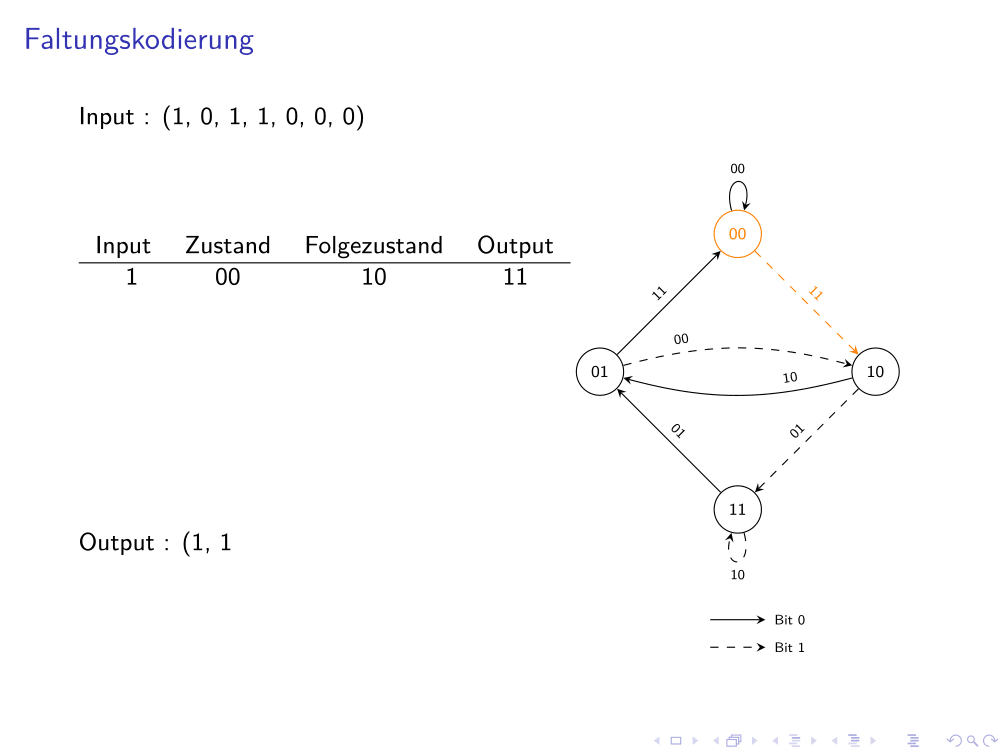
\includegraphics[width=0.99\textwidth]{abbildungen/folie_kodierung_2}}
		\caption{}
		\label{abb:folie_kodierung_2}
	\end{subfigure}
	
	\begin{subfigure}{0.65\textwidth}
		\centering
		\fbox{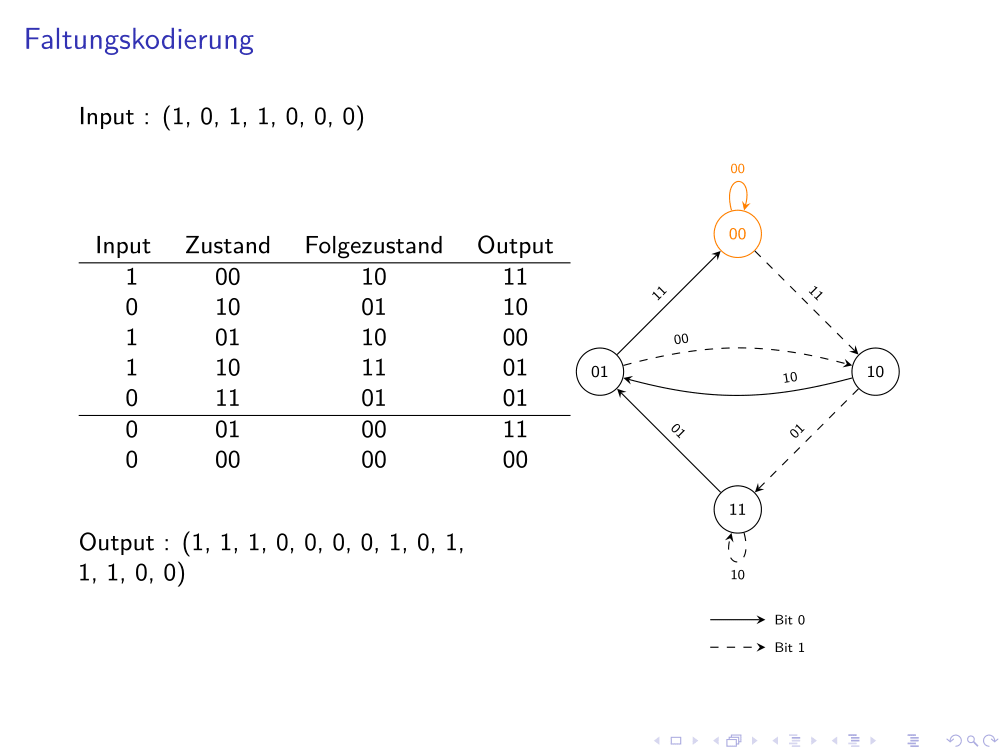
\includegraphics[width=0.99\textwidth]{abbildungen/folie_kodierung_3}}
		\caption{}
		\label{abb:folie_kodierung_3}
	\end{subfigure}
	\caption{Folien der Kodierung}
	\label{abb:folie_kodierung}
\end{figure}
Daraufhin folgt die Visualisierung der Kodierung. Dabei wird die zu kodierende Nachricht Bit für Bit auf einer eigenen Folie verarbeitet. Abbildung~\ref{abb:folie_kodierung} zeigt die ersten beiden Schritte sowie den letzten Schritt der Kodierung. In Abbildung~\ref{abb:folie_kodierung_1} ist die Folie vor der Kodierung des ersten Bits zu sehen. Zunächst ist die zu kodierende Nachricht (Input), das Zustandsübergangsdiagramm sowie eine noch nicht befüllte Kodierungstabelle zu sehen. Das Kodewort wird auf den folgenden Folien Schritt für Schritt erarbeitet. Durch diese Herangehensweise ist die Kodierung für den Benutzer einfach nachzuvollziehen. Abbildung~\ref{abb:folie_kodierung_2} zeigt den nächsten Schritt der Kodierung. Das erste Bit des Inputs, der aktuelle Zustand, Folgezustand sowie der resultierende Output wird in eine neue Zeile der Kodierungstabelle geschrieben. Der aktuelle Zustand sowie der entsprechende Übergang werden im Diagramm farblich hervorgehoben, um die Kodierung auch im Zustandsdiagramm verfolgen zu können. Der Output wird auch unterhalb der Tabelle eingetragen und wächst mit jedem Schritt bis schlussendlich die gesamte Nachricht kodiert wurde. Die Visualisierung am Ende der Kodierung ist in Abbildung~\ref{abb:folie_kodierung_3} zu sehen. Die Bits unterhalb der horizontalen Trennlinie stellen die Terminierungsbits dar.
\\
\\
% Kode zu Signal
\begin{figure}[t]
	\centering
	\fbox{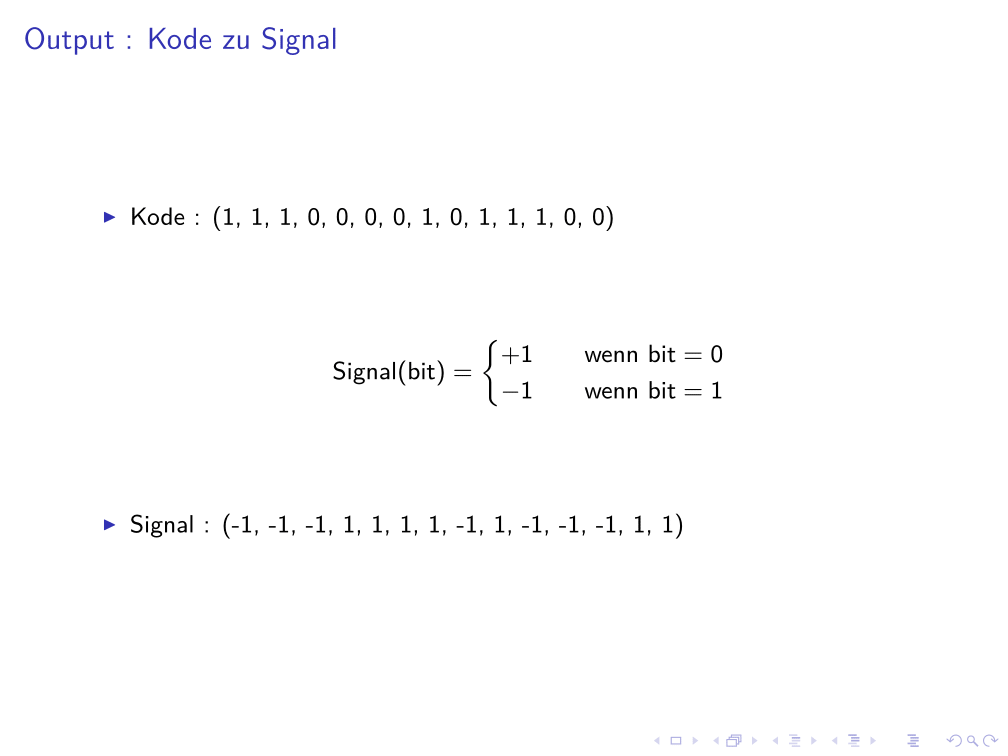
\includegraphics[width=0.65\textwidth]{abbildungen/folie_kodierung_bit_zu_signal}}
	\caption{Folie mit der Bit zu Signal Abbildung}
	\label{abb:folie_bit_zu_signal_abbildung}
\end{figure}
Da die Kodierungsfunktion nicht die Bitwerte des Kodeworts zurückliefert sondern die Signalwerte (für eine Übertragung über einen Kanal) wird auf einer weiteren Folie, wie in Abbildung~\ref{abb:folie_bit_zu_signal_abbildung} zu sehen, die Abbildung der Kodebits zu den Signalpegeln (nach Gleichung~\ref{eq:bit_zu_signal_abbildung}) dargestellt.
\\
\\
% Punktierung
\begin{figure}[t]
	\centering
	\fbox{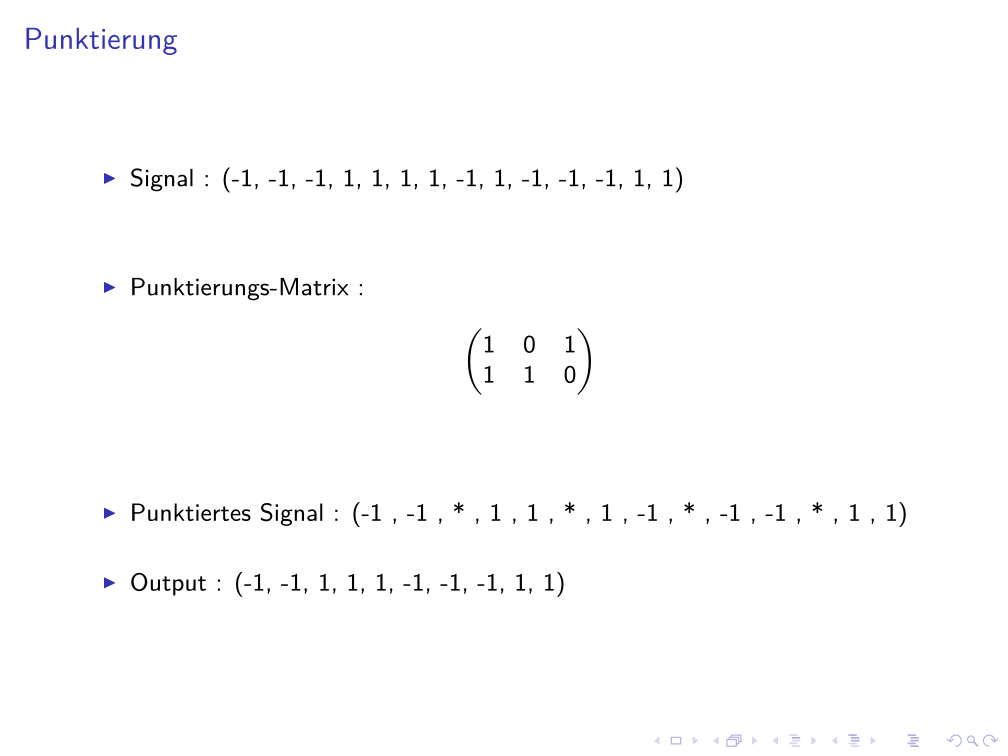
\includegraphics[width=0.65\textwidth]{abbildungen/folie_kodierung_punktierung}}
	\caption{Folie mit Punktierung}
	\label{abb:folie_punktierung}
\end{figure}
Abbildung~\ref{abb:folie_punktierung} zeigt die Folie der Punktierung. Auf dieser wird die Punktierung des Signals, d.h. das Entfernen von Signalwerten (definiert durch die Punktierungsmatrix) dargestellt. Dabei wird neben dem originalen Signal und der Punktierungsmatrix das punktierte Signal dargestellt, wobei zunächst die punktierten Signalwerte, d.h. die entfernten Werte, durch Asterisk-Symbole ($\ast$) ersetzt werden. Diese Darstellung dient als visueller Zwischenschritt für das danach folgende tatsächlich punktierte Signal, bei dem die punktierten Werte fehlen, was auch dem Rückgabewert der Funktion entspricht.

\section{Dekodierung}
\label{kapitel:visualisierung_dekodierung}
% allg. Informationen
Bei der Dekodierung befinden sich ebenfalls, wie bei der Kodierung, allgemeine Informationen des Faltungskodierers auf den ersten Folien.
\\
\\
% Depunktierung
\begin{figure}[th]
	\centering
	\fbox{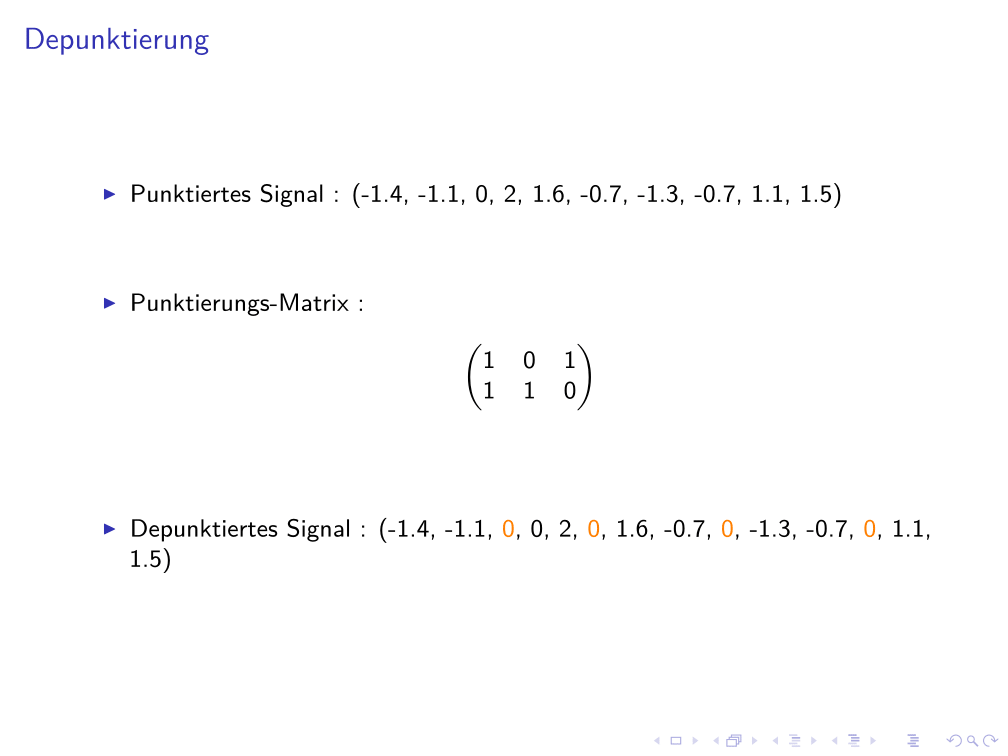
\includegraphics[width=0.65\textwidth]{abbildungen/folie_dekodierung_depunktierung}}
	\caption{Folie mit Depunktierung}
	\label{abb:folie_depunktierung}
\end{figure}
Abbildung~\ref{abb:folie_depunktierung} zeigt die Folie der Depunktierung. Auf dieser wird die Depunktierung des Signals, d.h. das Einfügen des Signalwerts 0 (definiert durch die Punktierungsmatrix), dargestellt. Die eingefügten 0-Werte sind zur leichteren visuellen Erkennung farblich hervorgehoben.
\\
\\
% Signal zu Kode
\begin{figure}[th]
	\centering
	\fbox{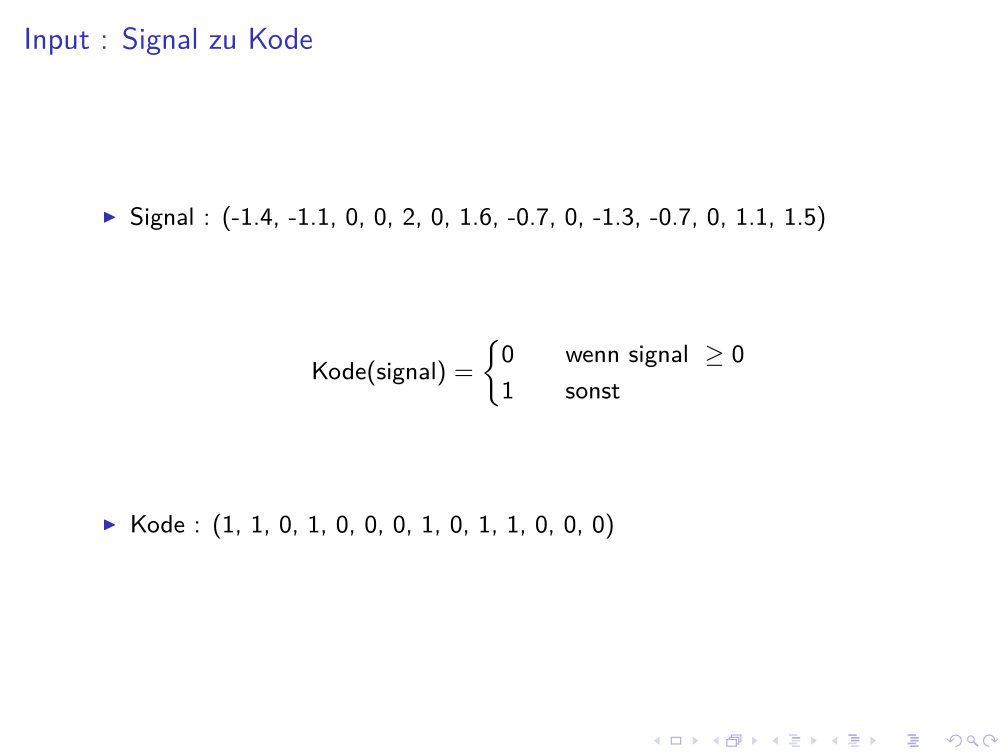
\includegraphics[width=0.65\textwidth]{abbildungen/folie_dekodierung_signal_zu_bit}}
	\caption{Folie mit der Signal zu Bit Abbildung}
	\label{abb:folie_signal_zu_bit_abbildung}
\end{figure}
Als Input erhält die Dekodierung das Kodewort als kontinuierliche Signalwerte, die möglicherweise durch Anwendung der \texttt{ApplyNoise} Funktion verfälscht worden sind. Die soft decision Dekodierung verwendet zur Dekodierung zwar direkt diese Signalwerte, da aber sowohl die hard decision Dekodierung Bitwerte zur Dekodierung verwendet und die Kanten des Trellis mit Bitwerten beschriftet sind, wird der Input, um konsistent zu bleiben, auf Bitwerte abgebildet. Die Folie der Abbildung der Signalwerte auf Bitwerte (nach Gleichung~\ref{eq:signal_zu_bit_abbildung}) ist in Abbildung~\ref{abb:folie_signal_zu_bit_abbildung} zu sehen.
\\
\\
% Viterbi-Algorithmus
\begin{figure}[th]
	\centering
	\begin{subfigure}{0.48\textwidth}
		\centering
		\fbox{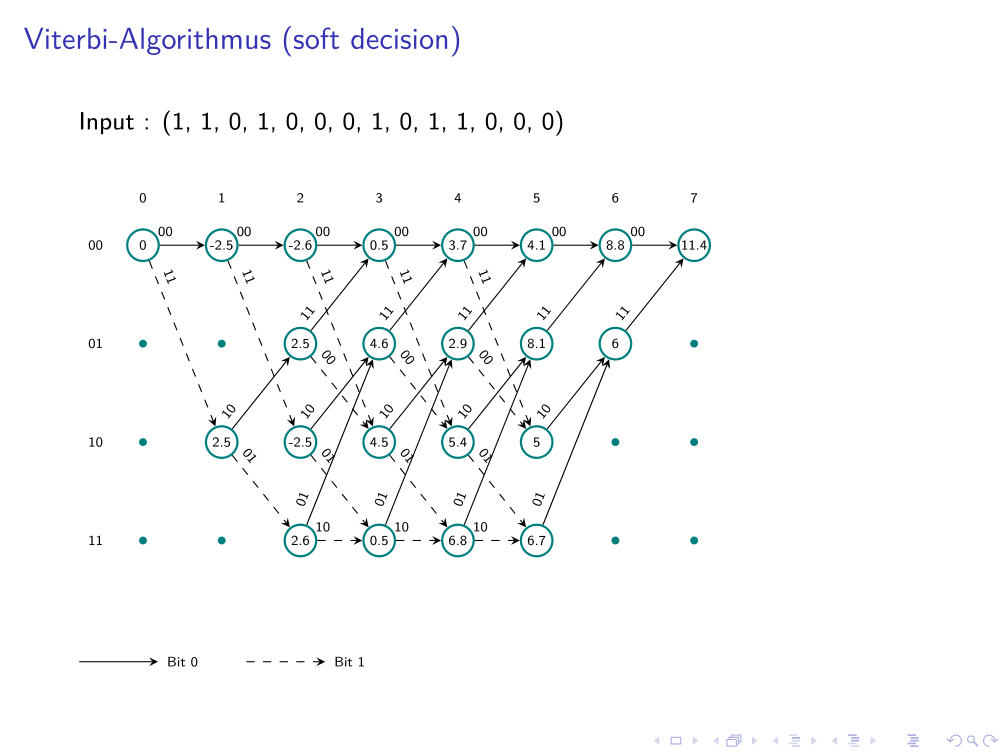
\includegraphics[width=0.99\textwidth]{abbildungen/folie_dekodierung_1}}
		\caption{}
		\label{abb:folie_dekodierung_1}
	\end{subfigure}
	\quad % spacing between subfigures
	\begin{subfigure}{0.48\textwidth}
		\centering
		\fbox{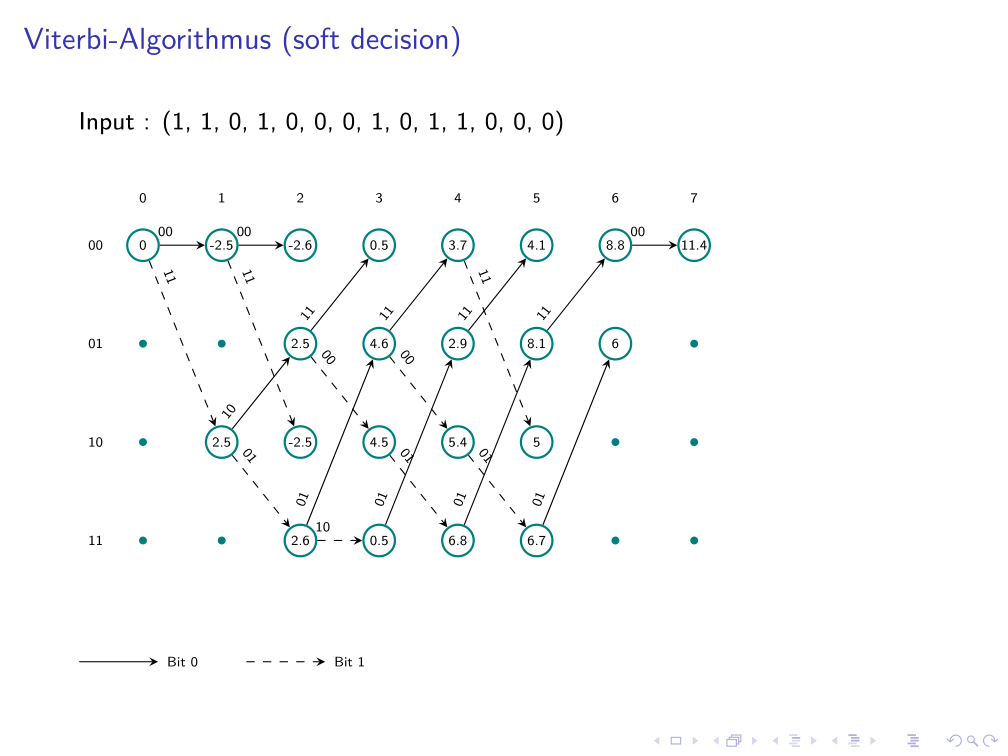
\includegraphics[width=0.99\textwidth]{abbildungen/folie_dekodierung_2}}
		\caption{}
		\label{abb:folie_dekodierung_2}
	\end{subfigure}
	
	\begin{subfigure}{0.48\textwidth}
		\centering
		\fbox{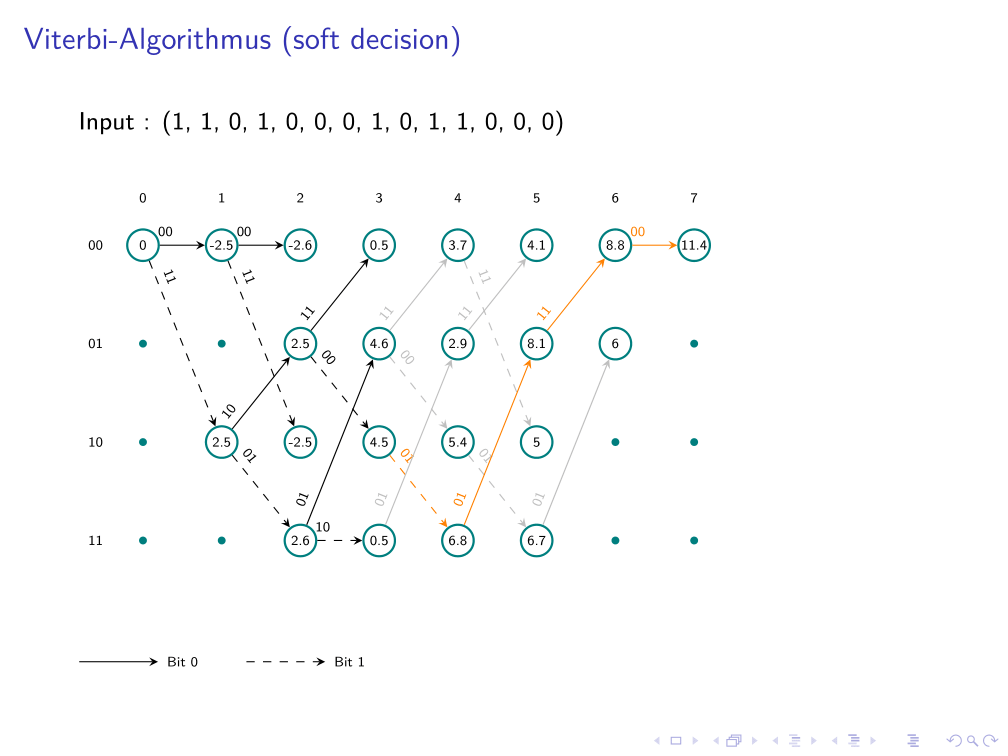
\includegraphics[width=0.99\textwidth]{abbildungen/folie_dekodierung_3}}
		\caption{}
		\label{abb:folie_dekodierung_3}
	\end{subfigure}
	\quad % spacing between subfigures
	\begin{subfigure}{0.48\textwidth}
		\centering
		\fbox{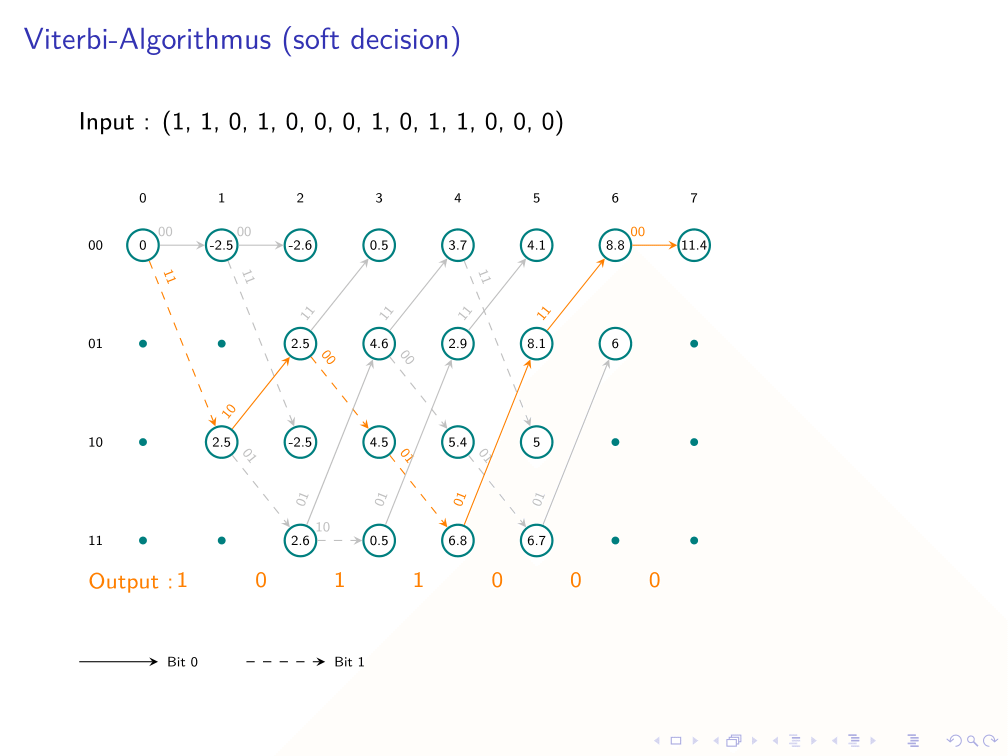
\includegraphics[width=0.99\textwidth]{abbildungen/folie_dekodierung_4}}
		\caption{}
		\label{abb:folie_dekodierung_4}
	\end{subfigure}
	\caption{Folien mit der soft decision Dekodierung}
	\label{abb:folie_dekodierung}
\end{figure}
Anschließend folgt die Visualisierung des Viterbi-Algorithmus mithilfe des Trellis-Diagramms. In den farbigen Kreisen befinden sich die Metriken der Pfade die zum jeweiligen Zustand führen. Zunächst werden, zur besseren Übersicht bei großen Diagrammen, jene Pfade entfernt, für die es eine bessere Alternative gibt. D.h. es werden jene Pfade entfernt die bei der soft decision Dekodierung eine niedrigere Metrik bzw. bei der hard decision Dekodierung eine höhere Metrik besitzen. Dieser Schritt ist zwischen den Abbildungen~\ref{abb:folie_dekodierung_1} und \ref{abb:folie_dekodierung_2} zu sehen. Danach erfolgt Schritt für Schritt mittels Backtracking die Rekonstruktion der Nachricht. Der gewählte Pfad beim Backtracking wird farblich hervorgehoben. Die übrigen Pfade werden ausgegraut. Eine Folie während des Backtrackings wird in Abbildung~\ref{abb:folie_dekodierung_3} veranschaulicht. Am Ende befindet sich unter dem Trellis-Diagramm die farblich hervorgehobene dekodierte Nachricht, wie in Abbildung~\ref{abb:folie_dekodierung_4} zu sehen ist. Die einzelnen Zwischenschritte vermitteln dem Benutzer wie der Algorithmus funktioniert und wie sich die dekodierte Nachricht ergibt.

\section{Simulation}
\label{kapitel:visualisierung_simulation}
Weiters können Berichte der Simulation generiert werden, die die resultierenden Daten u.a. in einem Diagramm darstellen.